\documentclass{article}
\usepackage{geometry}
\geometry{margin=1.5cm, vmargin={0pt,1cm}}
\setlength{\topmargin}{-1cm}
\setlength{\headheight}{12.5pt}
\setlength{\paperheight}{29.7cm}
\setlength{\textheight}{25.3cm}

% useful packages.
\usepackage[UTF8]{ctex}
\usepackage{fancyhdr}
\usepackage{layout}
\usepackage{luacode}

% import common macros
% % % % % % % % % % % % % % % % % % % % % % % % % % % % % % % %
% Common Macros for LaTeX
% % % % % % % % % % % % % % % % % % % % % % % % % % % % % % % %

% Useful packages
\usepackage{amsfonts}
\usepackage{amsmath}
\usepackage{amssymb}
\usepackage{amsthm}
\usepackage{enumerate}
\usepackage{graphicx}
\usepackage{multicol}
\usepackage[ruled,linesnumbered]{algorithm2e}

% Math operators and common symbols
\newcommand{\dif}{\mathrm{d}}
\newcommand{\innerProd}[1]{\left\langle #1 \right\rangle}
\newcommand{\difFrac}[2]{\frac{\dif #1}{\dif #2}}
\newcommand{\pdfFrac}[2]{\frac{\partial #1}{\partial #2}}
\newcommand{\T}{\mathrm{T}}
\newcommand{\norm}[1]{\left\| #1 \right\|}
\newcommand{\abs}[1]{\left| #1 \right|}

% Vector and Matrix shortcuts
\newcommand{\vecTwo}[2]{
  \begin{bmatrix}
    #1 \\
    #2
\end{bmatrix}}
\newcommand{\vecThree}[3]{
  \begin{bmatrix}
    #1 \\
    #2 \\
    #3
\end{bmatrix}}
\newcommand{\vecTwoH}[2]{
  \begin{bmatrix}
    #1 & #2
  \end{bmatrix}
}
\newcommand{\vecThreeH}[3]{
  \begin{bmatrix}
    #1 & #2 & #3
  \end{bmatrix}
}

% Common fields
\newcommand{\R}{\mathbb{R}}
\newcommand{\C}{\mathbb{C}}
\newcommand{\Q}{\mathbb{Q}}
\newcommand{\Z}{\mathbb{Z}}
\newcommand{\N}{\mathbb{N}}

% Common Operators
\renewcommand{\Re}{\mathrm{Re}}
\renewcommand{\Im}{\mathrm{Im}}

% Theorem-like environments
\theoremstyle{definition}
\newtheorem{theorem}{Theorem}[section]
\newtheorem{lemma}[theorem]{Lemma}
\newtheorem{corollary}[theorem]{Corollary}
\newtheorem{definition}[theorem]{Definition}
\newtheorem{remark}[theorem]{Remark}
\newtheorem{exercise}{Exercise}[section]

% Support for individual Chinese characters using fontspec (for LuaLaTeX)
\usepackage{fontspec}
\newfontfamily\zhfont{SimSun} % Search system fonts by name
\newcommand{\zhstr}[1]{{\zhfont #1}}

% Solutions and proofs
\AtBeginDocument{
  \ifdefined\ctexset
  \newenvironment{solution}{
  \begin{proof}[解]}{
  \end{proof}}
  \else
  \newenvironment{solution}{
  \begin{proof}[Solution]}{
  \end{proof}}
  \fi
}

\usepackage{luacode}
% Utility to get environment variables (requires lualatex)
\newcommand{\getEnv}[2]{\directlua{tex.print(os.getenv("#1") or "#2")}}


\usepackage{listings}
\usepackage{xcolor}

% Configure listings for Python code highlighting
\lstset{
  language=Python,
  basicstyle=\ttfamily\small,
  keywordstyle=\bfseries\color{blue},
  commentstyle=\color{gray},
  stringstyle=\color{red},
  breaklines=true,
  showstringspaces=false,
  tabsize=4,
  frame=single,
  framesep=5pt,
  rulecolor=\color{gray},
  backgroundcolor=\color{white},
  captionpos=b,
  numberstyle=\tiny\color{gray},
  numbers=left,
  stepnumber=5,
}

\lstnewenvironment{plaintext}[1][]{
  \lstset{
    language=none,
    basicstyle=\ttfamily,
    keywordstyle=,
    commentstyle=,
    stringstyle=,
    numbers=none,
    frame=none,
    backgroundcolor=\color{white},
    #1                % 允许用户自行覆盖默认设置
  }
}{}

% Name and uID
\newcommand{\name}{\getEnv{NAME}{NAME}}
\newcommand{\uid}{\getEnv{UID}{UID}}
\newcommand{\course}{数值代数}
\newcommand{\hwNum}{5}

\begin{document}

\pagestyle{fancy}
\fancyhead{}
\lhead{\name (\uid)}
\chead{\course \#\hwNum}
\rhead{\today}

\section{题目 1：谱范数性质}

设 $A \in \mathbb{R}^{n\times n}$，证明：

\begin{enumerate}
  \item $\|A\|_2 = \max\{ |y^{T}Ax| : x, y \in \mathbb{R}^n, \|x\|_2
    = \|y\|_2 = 1 \}$；
  \item $\|A^T\|_2 = \|A\|_2 = \sqrt{\|A^TA\|_2}$；
  \item 对于任意的 $n$ 阶正交矩阵 $U$ 和 $V$，有 $\|UA\|_2 = \|AV\|_2 = \|A\|_2$。
\end{enumerate}

\begin{proof}
  (1) 由谱范数的定义，$\|A\|_2 = \max_{\|x\|_2=1} \|Ax\|_2$。

  对于任意固定的 $x$，由向量范数的对偶性，有
  \[
    \|Ax\|_2 = \max_{\|y\|_2=1} |y^T Ax|.
  \]
  事实上，由 Cauchy-Schwarz 不等式，$|y^T Ax| \leq \|y\|_2 \|Ax\|_2 =
  \|Ax\|_2$，且当取 $y = Ax/\|Ax\|_2$ 时等号成立。

  因此
  \[
    \|A\|_2 = \max_{\|x\|_2=1} \|Ax\|_2 = \max_{\|x\|_2=1}
    \max_{\|y\|_2=1} |y^T Ax| = \max\{ |y^{T}Ax| : x, y \in
    \mathbb{R}^n, \|x\|_2 = \|y\|_2 = 1 \}.
  \]

  (2) 首先证明 $\|A\|_2 = \sqrt{\|A^TA\|_2}$。

  设 $A^TA$ 的特征值为 $\lambda_1 \geq \lambda_2 \geq \cdots \geq \lambda_n
  \geq 0$（因为 $A^TA$ 是对称半正定矩阵），对应的正交特征向量为 $v_1, \ldots, v_n$。

  对于任意单位向量 $x$，可表示为 $x = \sum_{i=1}^n c_i v_i$，其中 $\sum_{i=1}^n c_i^2 = 1$。于是
  \[
    \|Ax\|_2^2 = x^T A^T A x = \sum_{i=1}^n \lambda_i c_i^2 \leq
    \lambda_1 \sum_{i=1}^n c_i^2 = \lambda_1.
  \]
  当 $x = v_1$ 时取等号，故 $\|A\|_2^2 = \lambda_1$。

  另一方面，由于 $A^TA$ 是对称矩阵，其谱范数为
  \[
    \|A^TA\|_2 = \max_{\|x\|_2=1} |x^T A^T A x| = \lambda_1.
  \]
  因此 $\|A\|_2 = \sqrt{\lambda_1} = \sqrt{\|A^TA\|_2}$。

  再证明 $\|A^T\|_2 = \|A\|_2$。由上述结论，
  \[
    \|A^T\|_2^2 = \|(A^T)^T A^T\|_2 = \|AA^T\|_2.
  \]
  注意到 $AA^T$ 和 $A^TA$ 有相同的非零特征值。事实上，若 $\lambda \neq 0$ 是 $A^TA$
  的特征值，对应的特征向量为 $v$，即 $A^TAv = \lambda v$，则
  \[
    AA^T(Av) = A(A^TAv) = A(\lambda v) = \lambda (Av),
  \]
  且 $Av \neq 0$（否则 $A^TAv = 0$，矛盾）。因此 $\lambda$ 也是 $AA^T$ 的特征值。反之亦然。

  所以 $\|A^T\|_2^2 = \|AA^T\|_2 = \lambda_1 = \|A^TA\|_2 =
  \|A\|_2^2$，即 $\|A^T\|_2 = \|A\|_2$。

  (3) 先证 $\|AV\|_2 = \|A\|_2$。由于 $V$ 是正交矩阵，当 $x$ 取遍所有单位向量时，$Vx$ 也取遍所有单位向量。因此
  \[
    \|AV\|_2 = \max_{\|x\|_2=1} \|AVx\|_2 = \max_{\|y\|_2=1} \|Ay\|_2 = \|A\|_2,
  \]
  其中令 $y = Vx$。

  再证 $\|UA\|_2 = \|A\|_2$。由 (2) 的结论，
  \[
    \|UA\|_2^2 = \|(UA)^T(UA)\|_2 = \|A^T U^T U A\|_2 = \|A^T A\|_2 = \|A\|_2^2,
  \]
  其中用到 $U^TU = I$。因此 $\|UA\|_2 = \|A\|_2$。

  综上所述，$\|UA\|_2 = \|AV\|_2 = \|A\|_2$。\hfill $\square$
\end{proof}

\section{题目 2：二阶矩阵的范数与条件数}

设

\[
  A =
  \begin{pmatrix}
    1 & 2 \\
    -1 & 2
  \end{pmatrix},
\]

分别求出 $\|A\|_1$、$\|A\|_2$、$\|A\|_\infty$，以及相应的条件数
$\kappa_1(A)$、$\kappa_2(A)$、$\kappa_\infty(A)$。

\begin{solution}
  (1) 计算 $\|A\|_1$（列和范数）：
  \[
    \|A\|_1 = \max_{j} \sum_{i=1}^{2} |a_{ij}| = \max\{|1|+|-1|,
    |2|+|2|\} = \max\{2, 4\} = 4.
  \]

  (2) 计算 $\|A\|_\infty$（行和范数）：
  \[
    \|A\|_\infty = \max_{i} \sum_{j=1}^{2} |a_{ij}| = \max\{|1|+|2|,
    |-1|+|2|\} = \max\{3, 3\} = 3.
  \]

  (3) 计算 $\|A\|_2$（谱范数）：
  \[
    A^TA =
    \begin{pmatrix} 1 & -1 \\ 2 & 2
    \end{pmatrix}
    \begin{pmatrix} 1 & 2 \\ -1 & 2
    \end{pmatrix}
    =
    \begin{pmatrix} 2 & 0 \\ 0 & 8
    \end{pmatrix}.
  \]
  $A^TA$ 的特征值为 $\lambda_1 = 8$，$\lambda_2 = 2$，故
  \[
    \|A\|_2 = \sqrt{\lambda_{\max}(A^TA)} = \sqrt{8} = 2\sqrt{2}.
  \]

  (4) 计算条件数。首先求逆矩阵：
  \[
    \det(A) = 1 \times 2 - 2 \times (-1) = 4, \quad
    A^{-1} = \frac{1}{4}
    \begin{pmatrix} 2 & -2 \\ 1 & 1
    \end{pmatrix}.
  \]

  \textbf{1-范数条件数}：
  \[
    \|A^{-1}\|_1 = \max\left\{\frac{1}{2}+\frac{1}{4},
    \frac{1}{2}+\frac{1}{4}\right\} = \frac{3}{4},
    \quad \kappa_1(A) = \|A\|_1 \|A^{-1}\|_1 = 4 \times \frac{3}{4} = 3.
  \]

  \textbf{$\infty$-范数条件数}：
  \[
    \|A^{-1}\|_\infty = \max\left\{\frac{1}{2}+\frac{1}{2},
    \frac{1}{4}+\frac{1}{4}\right\} = 1,
    \quad \kappa_\infty(A) = \|A\|_\infty \|A^{-1}\|_\infty = 3 \times 1 = 3.
  \]

  \textbf{2-范数条件数}：由定义 $\kappa_2(A) = \|A\|_2 \cdot \|A^{-1}\|_2$。

  已知 $\|A\|_2 = \sqrt{8} = 2\sqrt{2}$。下面计算 $\|A^{-1}\|_2$：
  \[
    (A^{-1})^T A^{-1} = (A^T)^{-1} A^{-1} = (AA^T)^{-1}.
  \]
  由于 $AA^T$ 与 $A^TA$ 有相同的非零特征值（即 8 和 2），故 $(AA^T)^{-1}$ 的特征值为 $1/8$ 和 $1/2$。因此
  \[
    \|A^{-1}\|_2 = \sqrt{\lambda_{\max}((AA^T)^{-1})} =
    \sqrt{\frac{1}{2}} = \frac{1}{\sqrt{2}}.
  \]
  于是
  \[
    \kappa_2(A) = \|A\|_2 \cdot \|A^{-1}\|_2 = 2\sqrt{2} \times
    \frac{1}{\sqrt{2}} = 2.
  \]
\end{solution}

\section{题目 3：三阶矩阵的范数与条件数}

设

\[
  A =
  \begin{pmatrix}
    -2 & 1 & 0 \\
    1 & -2 & 1 \\
    0 & 1 & -2
  \end{pmatrix},
\]

求 $\|A\|_1$、$\|A\|_2$、$\|A\|_\infty$ 和条件数 $\kappa_2(A)$。

\begin{solution}
  注意到 $A$ 是对称矩阵，即 $A^T = A$。

  (1) 计算 $\|A\|_1$（列和范数）：
  \[
    \|A\|_1 = \max\{|{-2}|+1+0, 1+|{-2}|+1, 0+1+|{-2}|\} = \max\{3, 4, 3\} = 4.
  \]

  (2) 计算 $\|A\|_\infty$（行和范数）：
  \[
    \|A\|_\infty = \max\{|{-2}|+1+0, 1+|{-2}|+1, 0+1+|{-2}|\} =
    \max\{3, 4, 3\} = 4.
  \]

  (3) 计算 $\|A\|_2$ 和 $\kappa_2(A)$：

  由于 $A$ 是对称矩阵，$\|A\|_2 = \max_i |\lambda_i|$，其中 $\lambda_i$ 为 $A$ 的特征值。

  计算 $A$ 的特征值：
  \[
    \det(A - \lambda I) =
    \begin{vmatrix} -2-\lambda & 1 & 0 \\ 1 & -2-\lambda & 1 \\ 0 & 1
      & -2-\lambda
    \end{vmatrix} = 0.
  \]
  解得 $\lambda_1 = -2 - \sqrt{2}$，$\lambda_2 = -2$，$\lambda_3 = -2 + \sqrt{2}$。

  因此
  \[
    \|A\|_2 = \max_i |\lambda_i| = |-2-\sqrt{2}| = 2 + \sqrt{2}.
  \]

  对于对称矩阵，$\kappa_2(A) = \frac{|\lambda|_{\max}}{|\lambda|_{\min}}$，故
  \[
    \kappa_2(A) = \frac{2+\sqrt{2}}{2-\sqrt{2}} =
    \frac{(2+\sqrt{2})^2}{4-2} = \frac{6+4\sqrt{2}}{2} = 3 + 2\sqrt{2}.
  \]
\end{solution}

\section{上机习题 1：Hilbert 矩阵条件数}

先用你所熟悉的计算机语言将算法 2.5.1 编制成通用的子程序，然后再用你所编制的子程序估计 $5$ 到 $20$ 阶 Hilbert
矩阵的 $\infty$ 范数条件数。

\begin{solution}
  \mbox{}
  \lstinputlisting[language={},caption={上机习题 1 的输出结果}]{prob1-out.txt}
  从输出结果可以看出，随着 Hilbert 矩阵阶数的增加，其 $\infty$ 范数条件数呈指数级增长，这表
  明 Hilbert 矩阵是一个非常病态的矩阵，尤其在高阶时数值稳定性极差。这里我们采用了三种方式进行
  计算：理论推导出来的 Hilbert 矩阵条件数的解析公式、数值方法以及 NumPy 库提供的数值方法。通
  过比较三者的结果，我们可以看到数值方法在较小阶数时能够较好地近似解析结果，但随着阶数的增加，
  数值方法的误差也逐渐增大，尤其是当阶数超过 15 时，数值方法的结果与解析结果之间的差距明显增大。
  这进一步说明了 Hilbert 矩阵在高阶时的病态性质，以及数值方法在处理病态矩阵时可能面临的挑战。
  \begin{center}
    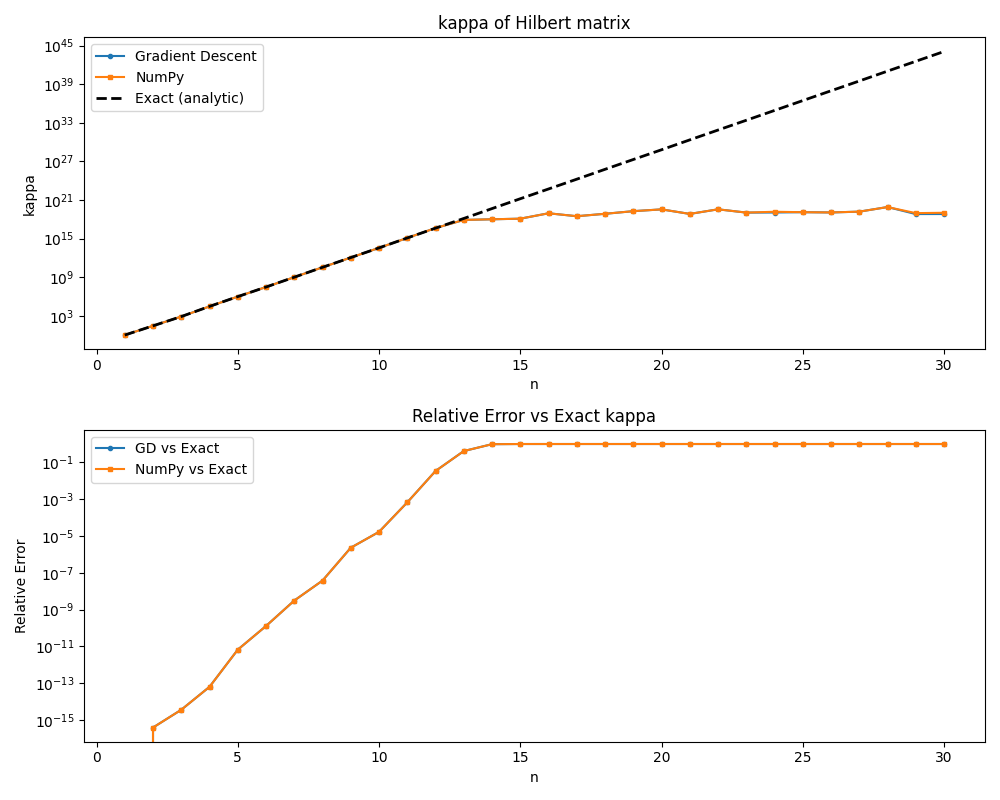
\includegraphics[width=0.8\textwidth]{kappa_comparison.png}
  \end{center}
\end{solution}

\section{上机习题 2：列主元 Gauss 消去法误差分析}

设

\[
  A_n =
  \begin{bmatrix}
    1 & 0 & \cdots & 0 & 1 \\
    -1 & \ddots & \ddots & \vdots & \vdots \\
    \vdots & \ddots & \ddots & 0 & 1 \\
    -1 & \cdots & -1 & 1 & 1 \\
    -1 & \cdots & -1 & -1 & 1
  \end{bmatrix}
  \in \mathbb{R}^{n\times n}.
\]

先随机地选取 $x \in \mathbb{R}^n$，并计算 $b = A_n x$；然后再用列主元 Gauss
消去法求解该方程组，假定计算解为 $\hat{x}$。试对 $n$ 从 $5$ 到 $30$ 估计计算解 $\hat{x}$ 的精度，并且与真实相对误差作比较。

\begin{solution}
  \mbox{}
  \lstinputlisting[language={},caption={上机习题 2 的输出结果}]{prob2-out.txt}
  \begin{center}
    
\includegraphics[width=0.8\textwidth]{accuracy_comparison.png}
  \end{center}
  可以看到二者的误差都随着 $n$ 的增加而增加，且增长情况几乎一样。可见这种误差估计可以有效地估计
  真实误差的上界，且在 $n$ 较小时二者几乎一致。
\end{solution}

\section*{上机习题代码}

\lstinputlisting[language=Python,caption={两道上机习题的完整代码}]{kappa.py}

\end{document}
